% ===========================================================================
% Title:
% ---------------------------------------------------------------------------
% to create Type I fonts type "dvips -P cmz -t letter <filename>"
% ===========================================================================
\documentclass[11pt]{article}       %--- LATEX 2e base
\usepackage{latexsym}               %--- LATEX 2e base
\usepackage[table]{xcolor}
\usepackage{tikz}
\usetikzlibrary{shapes}
\usepackage{forest}
\usepackage{adjustbox}
\usepackage{amsmath}
\usepackage{pgfplots}
%---------------- Wide format -----------------------------------------------
\textwidth=6in \textheight=9in \oddsidemargin=0.25in
\evensidemargin=0.25in \topmargin=-0.5in
%---------------- Custom Colors -----------------------------------------------
\definecolor{darkGreen}{HTML}{186A3B}
\definecolor{orange}{HTML}{D35400}
%--------------- Def., Theorem, Proof, etc. ---------------------------------
\newtheorem{definition}{Definition}
\newtheorem{theorem}{Theorem}
\newtheorem{lemma}{Lemma}
\newtheorem{corollary}{Corollary}
\newtheorem{property}{Property}
\newtheorem{observation}{Observation}
\newtheorem{fact}{Fact}
\newenvironment{proof}           {\noindent{\bf Proof.} }%
                                 {\null\hfill$\Box$\par\medskip}
%--------------- Algorithm --------------------------------------------------
\usepackage[ruled, lined, vlined, linesnumbered]{algorithm2e}
%--------------- Figures ----------------------------------------------------
\usepackage{graphicx}

\newcommand{\includeFig}[3]      {\begin{figure}[htb] \begin{center}
                                 \includegraphics
                                 [width=4in,keepaspectratio] %comment this line to disable scaling
                                 {#2}\caption{\label{#1}#3} \end{center} \end{figure}}
                                 % usage: \includeFig{label}{file}{caption}


% ===========================================================================
\begin{document}
% ===========================================================================

% ############################################################################
% Title
% ############################################################################

\title{Top Down Specialization on Apache Spark\texttrademark}


% ############################################################################
% Author(s) (no blank lines !)
\author{
% ############################################################################
Macarious Abadeer\\
School of Computer Science\\
Carleton University\\
Ottawa, Canada K1S 5B6\\
{\em macariousabadeer@cmail.carleton.ca}
% ############################################################################
} % end-authors
% ############################################################################

\maketitle

% ############################################################################
% Abstract
% ############################################################################
\begin{abstract}
This paper provides an implementation of Top-Down Specialization algorithm for data anonymization in parallel using Apache Spark. It evaluates the performance on large datasets of up to 20-million rows in a variety of different cluster environments.
\end{abstract}


% ############################################################################
\section{Introduction} \label{intro}
% ############################################################################

Since the introduction of multi-core processors in 2004 by Intel\textsuperscript{\textregistered}, parallel computing evolved to exploit the advantages of multiple processing units that became the norm for personal computers. This evolution was also expanded and accelerated by the advancements in Cloud Computing that supported running compute-intensive applications over a network of clusters. Parallel computing enabled the development of solutions to different real world applications that were hindered by scalability limitations such as big data analytics, machine learning and artificial intelligence. One of the problems that parallel computing provided scaleable solutions for is data anonymization, especially for big data. 

In today's abundance of big data ranging from retail and banking transactions, health care, social media interactions and sensor data, a need was created for measures that protect people's most private and sensitive data. One of the most popular theories that were developed in this area was $k$-anonymity developed by Samarati and Sweeney in 1998 \cite{Samarati-P.:1998}. Sweeney argued that an individual in a dataset can be identified when the dataset is linked with other public datasets even if the original dataset did not contain identifying information such as name, date of birth and social insurance number. Sweeney was able to show that when linking voter registration cards and health care data, individuals can be identified with 87\% accuracy. Those potentially identifying attributes are called Quasi-Identifiers (QID). $k$-anonymity states that a dataset is called $k$-anonymous when for a given record, there exists at least \(k-1\) records in the same dataset with the same QID values.  Further modifications to $k$-anonymity were made to overcome its shortcomings such as introducing $\ell$-diversity \cite{Machanavajjhala:2007} and $t$-closeness \cite{Li-N.:2007}. $\ell$-diversity ensures that sensitive attributes, such as diagnosis in a health care dataset, need to have diverse values so that an adversary with foreknowledge of a given QID set cannot deduce their diagnosis. $t$-closeness ensures that the distribution of these diverse values is close to their distribution in the original dataset.

While these theories contributed immensely to the practices of data anonymization, $k$-anonymity was proven to be $\mathcal{NP}$-hard by Meyerson and Williams \cite{Meyerson:2004}. Further research used these models as a baseline to develop scalable parallel algorithms that can handle big data.

The paper is organized as follows: in Section~\ref{literature}, I will go over the different ideas that were proposed to optimize and scale $k$-anonymity. Section~\ref{solution} will detail an implemented proposed solution and Section~\ref{evaluation} presents the experimentation results of the algorithm and the paper finally concludes in Section~\ref{conclusion}.

% ############################################################################
\section{Literature Review} \label{literature}
% ############################################################################

There are three different masking types that are used to satisfy $k$-anonymity: interval, taxonomy tree and suppression \cite{Al-Zobbi-Mohammed:2018}. Suppression requires certain outlier tuples to be removed to satisfy $k$-anonymity \cite{Samarati-P.:1998}. Intervals and taxonomy trees are generalization techniques applied to numerical and categorical attributes respectively \cite{Samarati-P.:1998}. For example two records with birth year of 1971 and 1973 can be generalized to 1970-1975. For a taxonomy tree, a categorical attribute such as education level can have, for example, post-graduate as a parent node which can have PhD, Masters and Post Graduate Diploma as its child leaves so that records with these values can be generalized to the parent node. The majority of research papers on anonymization with respect to big data involved taxonomy trees thus this is where I focus my literature survey.

One of the techniques that researchers attempted to optimize was Bottom-Up Generalization (BUG) which involves traversing the taxonomy tree of attribute hierarchies from the bottom (most specific) upwards (most general) \cite{Ke-Wang:2004}. Wang suggested that the taxonomy tree would be provided by the data supplier or the data recipient \cite{Ke-Wang:2004}. As the tree is traversed, two metrics are calculated to ensure a high quality generalization: information loss and anonymity gain. An indexed approach to bottom-up generalization was proposed by Hoang \cite{Hoang:2012} where the taxonomy tree for numerical attributes was generated automatically at runtime. Hoang's indexed approach could also handle numerical as well as categorical attributes. Indexed BUG starts with collecting statistical information about the dataset as well as partition it so it can be used in the generalization step which was further broken down to four steps: calculate the best generalization score based on the least information loss, calculate $k$-anonymity for every partition, generate an indexed generalization map which maps every value to its generalized value, and the last step creates the anonymized dataset using this map. Hoang's experiments showed that the generalization time did not increase with the dataset size due to the use of indexed generalization map however performance was impacted by the distinct values count for each QID \cite{Hoang:2012}.

Parallel BUG was introduced to address the limitations of traditional and indexed BUG approaches. Pandilakshmi attempted to solve the limitations of indexing structures since they are centralized and hard to parallelize and cannot run on distributed systems such as the Cloud \cite{Pandilakshmi:2014}. Pandilakshmi introduced Bi-Level BUG algorithm where MapReduce framework was used to take advantage of job-level and task-level parallelization. Job-level parallelization was achieved by using multiple MapReduce jobs and task-level parallelization was achieved by using multiple mapper/reducer tasks for every MapReduce job so they are executed in parallel on every partition. Data is partitioned according to a random number generated between 1 and $p$ where $p$ is the number of partitions. Pandilakshmi then runs MapReduce BUG driver (MRBUG) iteratively on the partitioned datasets and calculates generalization score (least information loss with the most anonymity gain) and stops until it finds the best generalization with the highest score that satisfies $k$-anonymity. Pandilakshmi experiments performed on varying datasets of up to 3GB showed that execution time was virtually capped at $\approx$33 minutes regardless of dataset size.

Another technique is Top-Down Specialization (TDS). TDS traverses the taxonomy tree from the top downwards where it starts with the most generalized values and specializes the value and stops when it violates $k$-anonymity \cite{Fung:2005}. Multiple solutions have been developed such as a scalable two-phase TDS introduced by \cite{Priyanka:2014} and \cite{Zhang:2014}. The first phase involves partitioning the original dataset to $p$ partitions using random sampling. A MapReduce TDS job runs in parallel on each partition. Each job specializes the data iteratively while calculating information gain and privacy loss metrics and creates an intermediate anonymized dataset. In the second phase the intermediate datasets are merged and further anonymized if necessary to satisfy $k$-anonymity. In \cite{Zhang:2014}, Zhang et al. adopted Hadoop\textsuperscript{\textregistered} and took advantage of distributed cache capability to pass the intermediate anonymized dataset to each mapper/reducer node. The experiments for this solution showed an overhead in the partitioning phase of the dataset.

A hybrid approach of BUG and TDS using MapReduce was introduced by \cite{Zhang:2013} where it was shown that when either TDS or BUG were used individually, they performed poorly for certain values of $k$. The hybrid approach applies TDS for large $k$ values and BUG for smaller ones. The notion of Workload Balancing Point was introduced which is defined as the point where the amount of computation required for TDS is the same as BUG. Once that point is identified, the hybrid approach chooses TDS for $k$ greater than the workload balancing point and chooses BUG when $k$ is smaller. The workload balancing point is estimated using the height of the taxonomy tree as a reference.

Al-Zobbi et al \cite{Al-Zobbi-Mohammed:2018} argued that finding the highest scoring generalization and specialization based on information gain and anonymity loss in BUG and TDS require high computational costs and impedes the ability to parallelize them. Al-Zobbi also argued that as the data grows in size, the high accuracy of these computations no longer make a statistical difference. Al-Zobbi proposed a multi-dimensional sensitivity-based algorithm on Apache Spark that uses a pre-determined QID attributes to anonymize as well as precalculated $k$ value using linear regression. The solution also takes into consideration the probability value of each QID. For example assuming that age can range between 1 and 100, the probability of finding a given age is 1\% which is much higher than a probability of finding a given job title assuming there are 200 different job titles. The solution prioritized the anonymization of higher probability attributes instead of calculating information gain and anonymity loss scores for every attribute. The solution also used a role-based access control equivalent system to set $k$ based on context. For example a health care dataset maybe given a lower $k$ (less anonymization) when shared with a doctor but a higher $k$ value when shared with an insurance risk analyst. The solution was implemented on Spark and aimed at minimizing the use of User Defined Functions (UDFs) since they run outside of the Spark JVM which is beyond the resource negotiator's control. Al-Zobbi recognized that this solution would sacrifice the analytical value of the dataset for the performance improvement gained by not calculating the best generalization options.

In a research paper by \cite{Shi:2015}, a survey was done on MapReduce vs. Spark for big data analytics. It concluded that Spark is better suited for problems that require accessing the same dataset multiple times such as the case with both TDS, BUG and their variants. The constant read and write by Hadoop to HDFS (Hadoop Distributed File System) is considered a significant overhead however Spark operates on datasets in memory and provides the capability of caching Resilient Distributed Datasets (RDDs) for faster access making it suitable for iterative algorithms. The experiments carried out by Shi et al in \cite{Shi:2015} found that Spark is 5 times faster than MapReduce for iterative algorithms regardless of data size.

Shi's findings in \cite{Shi:2015} are inline with other researchers that implemented anonymization algorithms on Spark such as \cite{Canbay:2017} and \cite{Sopaoglu:2017}. For example, \cite{Sopaoglu:2017} proposed a TDS implementation for Apache Spark that partitioned the dataset to $p$ partitions on $n$ Spark nodes where \(n=p\). The master node partitions the data and calculates the scores required by TDS such as information gain and privacy loss. The scores are sent to the driver node which performs aggregations required by further iterations until $k$ is satisfied. The experiments carried out for this solution by \cite{Sopaoglu:2017} showed that there is an overhead cost incurred when having more than one partition in a single node. The experiments also showed performance gains regardless of $k$ values and dataset sizes as long as Spark nodes are increased with the dataset size. As outlined by \cite{Al-Zobbi-Mohammed:2018}, ideally the partitioned dataset needs to fit in the node's memory in order to avoid spilling to disk.

The previously mentioned solutions are generic enough to be applied to any type of datasets. However, multiple other solutions have been proposed to address specific anonymization scenarios. I briefly include them here due to their relevance in terms of parallelization techniques. Parameshwarappa \cite{Parameshwarappa:2019} for example proposed a solution to anonymize physical activity collected by wearable gadgets. It uses a multi-level clustering algorithm based on Maximum Distance to Average Vector (MDAV). It attempts to cluster data points so that every cluster satisfies $k$-anonymity. If a cluster does not satisfy $k$-anonymity, differential privacy technique is used to add statistical noise to the cluster in a way that does not skew the analytical value of the dataset. 

Another solution was implemented to provide a parallel anonymization of transaction data such as retail and banking datasets in \cite{Memon:2015}. It uses an algorithm known as RBAT on MapReduce which uses set-based generalization to anonymize data based on user-provided set of rules. It partitions data in a way that ensures the workload of every partition is approximately the same across different partitions. The solution scans the whole dataset in order to achieve this efficient partitioning based on QID values to minimize data shuffling across partitions.

Other frameworks were also developed to address specific variations to $k$-anonymity mentioned such as $t$-closeness introduced by \cite{Li-N.:2007}. For example, \cite{Chakravorty:2017} developed a framework called Incognito using MapReduce that generates a distribution of sensitive attributes based on their count in the dataset. Given the frequency histogram generated, subsets of the sensitive attribute values that have the same parent in the taxonomy tree are put together in the same data bucket. The tree is sorted from left to right nodes in an ascending order of their frequencies in the generated histogram. The anonymized dataset is then mapped to the generated tree in order to ensure anonymized dataset is close to the original dataset in terms of distribution of values.

% ############################################################################
\section{Problem Statement} \label{problem}
% ############################################################################

This paper tackles the scalability of anonymization algorithms for Big Data specifically Top Down Specialization algorithm. There was only a handful of papers in the literature reviewed in Section~\ref{literature} that implemented anonymization algorithms on Spark and only one that implemented Top Down Specialization \cite{Sopaoglu:2017}. In that implementation the performance was assessed only up to 500 MB of data which is relatively small in the context of Big Data. This paper aims to assess the performance of Top Down Specialization on Spark for datasets larger than 500 MB. It will also use number of records as the gauge instead of size on disk. The question I aim to answer, how does Top Down Specialization scale up for datasets larger than 5 million rows or 500 MB? Are there any optimizations that can be done to improve speedups?

% ############################################################################
\section{Proposed Solution} \label{solution}
% ############################################################################

\subsection{Introduction to $k$-anonymity}

First, it is important to review definitions that will be used throughout this paper:

\begin{definition}[$k$-anonymity]
A dataset is called $k$-anonymous if for every record there exists at least \(k-1\) other records with the same Quasi-Identifier values. 
\end{definition}

\begin{definition}[Quasi-Identifiers]
Quasi-Identifiers are attributes that do not directly identify an individual, but when used together and linked with other datasets they have the potential of identifying an individual. They will be referred to as $QID$ throughout the paper.
\end{definition}

\begin{definition}[Sensitive Attributes] 
Sensitive Attributes are attributes that should remain private so an adversary cannot deduce their values. They will be referred to as $SA$ throughout the paper.
\end{definition}

\begin{definition}[Taxonomy Trees]
Taxonomy Trees are logical hierarchies of distinct values in a dataset.
\end{definition}

For example, in Table~\ref{table1} \emph{Education}, \emph{Gender} and \emph{City} are examples of $QID$s while \emph{Income} is an example of $SA$. Table~\ref{table1} does not satisfy $k$-anonymity since there are two unique records with the same $QID$ values. In this case an adversary with foreknowledge of the existence of an Orleans Male with a Master's degree in the dataset will be able to deduce the individual's income. The two records violating $k$-anonymity are highlighted in Table~\ref{table1}.

\begin{table}[htp]
\begin{center}
\begin{tabular}{|c|c|c|c|}
\hline
Education & Gender & City & Income \\
\hline
Grade 12 & Female & Nepean & \$65,000 \\
Bachelor's & Male & Ottawa & \$50,000 \\
\rowcolor [HTML]{EAECEE} Master’s & Male & Orleans & \$50,000 \\
\rowcolor [HTML]{EAECEE} PhD & Male & Gloucester & \$100,000 \\
Grade 12 & Female & Nepean & \$80,000 \\
Associate & Female & Kanata & \$90,000 \\
Associate & Female & Kanata & \$105,000 \\
Bachelor's & Male & Ottawa & \$50,000 \\
\hline
\end{tabular}
\end{center}
\caption{Dataset violating $k$-anonymity}
\label{table1}
\end{table}

Figure~\ref{taxonomyTree} represents a taxonomy tree for \emph{Education} column. The leaf nodes in the tree represent the distinct values present in the dataset. Taxonomy trees are provided by either the data provider or the data recipient for all $QID$ in the dataset. The root node of all taxonomy trees is \emph{Any}.

\begin{figure}[htp]
\begin{adjustbox}{width=\textwidth, center}
\begin{forest}
for tree={rectangle, edge={->,>=latex}, draw, align=center}
[Any,thick [Without-Post-Secondary [Preschool] [Elementary [1st-4th] [5th-6th] [7th-8th]] [Secondary [Junior-Secondary [9th] [10th]] [Senior-Secondary [11th] [12th] [HS-grad]]]] [Post-secondary [Some-college] [Assoc [Assoc-acdm] [Assoc-voc]] [University [Bachelors] [Prof-school] [Post-grad [Masters] [Doctorate]]]]]
\end{forest}
\end{adjustbox}
\caption{Education Taxonomy Tree}
\label{taxonomyTree}
\end{figure}

\subsection{Introduction to Top Down Specialization} \label{tdsIntro}

Top Down Specialization algorithm begins by removing all non $QID$s from the dataset. The resulting dataset is then grouped by $QID$ and $SA$ and the count is calculated for every group. A set of trees called Anonymization Cuts \{$AC$\} is created where it initially contains the taxonomy trees of all $QID$. The $AC$ represents the level of the taxonomy tree to which each $QID$ value will be generalized. The algorithm starts with generalizing all values to the root of the corresponding $AC$. The basic idea of the algorithm is that it starts from the top of the taxonomy tree and specializes the values until $k$ is violated. However, it does not simply specialize all attributes. It calculates a score for every $AC$ and only specializes the $AC$ with the highest score. The score which is shown in Equation~\ref{score} calculates the information gain per privacy loss for every $AC$. In other words, which $AC$ will provide the best information gain and the least privacy loss. Information gain involves calculating the entropy as well as counting all the values that get generalized to the $AC$'s root (\(|R_\nu|\)), the count of all values that get generalized to the $AC$'s root's children (\(|R_{\nu c}|\)), the count of all values that get generalized to the root for each value in \{$SA$\} and finally the count of all values that get generalized to $AC$'s root's children for each value in \{$SA$\}. The whole equation is shown in Equation~\ref{infoGain} below. The privacy loss involves calculating $k$ before specialization minus $k$ after specialization. The reason for this is that as we specialize values along the $AC$ trees, the data becomes more useful yet less private. The privacy loss equation is shown in Equation~\ref{privacyLoss}. Once the score is calculated, the root $AC$ with the highest score is removed from \{$AC$\} and its children are added as separate trees to the set of \{$AC$\}. That is, $AC$ tree is specialized one level lower. The algorithm re-iterates with the new set of \{$AC$\} until $k$ is violated. The values in the dataset are finally generalized to the root of the final \{$AC$\} set and that represents the anonymized dataset.

\begin{equation}
Score(\nu) = \begin{cases}
\frac{InfoGain(\nu)} {PrivacyLoss(\nu)} & PrivacyLoss(\nu) \neq 0\\
InfoGain(\nu) & otherwise
\end{cases}
\label{score}
\end{equation}

\begin{equation}
InfoGain(\nu) = I(R_\nu) - \sum\limits_{\text{$c$} \in children(\nu)} \frac{|R_{\nu\text{$c$}}|}{|R_\nu|} I(R_{\nu\text{$c$}})
\label{infoGain}
\end{equation}

\begin{equation}
I(R_\nu) = - \sum\limits_{sv \in \text{\{$SA$\}}} \frac{| R_{\nu\text{$sv$}} |}{ | R_\nu |} \times \log_2 \frac{| R_{\nu\text{$sv$}} |}{ | R_\nu |}
\label{entropy}
\end{equation}

\begin{equation}
PrivacyLoss(\nu) = |R_\nu| - \min(\{|R_{\nu c}|\})
\label{privacyLoss}
\end{equation}

\begin{table}[htp]
\begin{center}
\begin{tabular}{|c|c|c|c|c|}
\hline
Education & Gender & Age & Income & count \\
\hline
9th & M & 30 & $\leq \text{50k}$ & 3 \\
10th & M & 32 & $\leq \text{50k}$ & 4 \\
11th & M & 35 & $> \text{50k}$ & 2 \\
11th & M & 35 & $\leq \text{50k}$ & 3 \\
12th & F & 37 & $> \text{50k}$ & 3 \\
12th & F & 37 & $\leq \text{50k}$ & 1 \\
\hline
Bachelors & F & 42 & $> \text{50k}$ & 4 \\
Bachelors & F & 42 & $\leq \text{50k}$ & 2 \\
Bachelors & F & 44 & $> \text{50k}$ & 4 \\
Masters & M & 44 & $> \text{50k}$ & 4 \\
Masters & F & 44 & $> \text{50k}$ & 3 \\
Doctorate & F & 44 & $> \text{50k}$ & 1 \\
\hline
\end{tabular}
\end{center}
\caption{Calculating best score}
\label{table2}
\end{table}

Fung et. al provided an example in \cite{Fung:2005} which helps illustrate the calculations. I include it here for completeness. Using Table~\ref{table2} as our dataset, \emph{SA} in this case is the \emph{Income} attribute. $AC$ element to score is the $Education$ taxonomy tree shown in Figure~\ref{taxonomyTree} with $Any$ at its root. Calculating the score of this particular $AC$ is shown below:

\begin{table}[htp]
\begin{adjustbox}{width=\textwidth, center}
\begin{tabular}{|c|c|c|}
\hline
Operand & Description & Value\\
\hline
$| R_\nu |$ & Sum of counts of $Education$ attribute when generalized to \emph{Any} & 34\\
$| R_{\nu sv} |$ & Sum of counts of $Education$ attribute when generalized to \emph{Any} and \emph{SA} is \(>50k\) & 21\\
$| R_{\nu sv} |$ & Sum of counts of $Education$ attribute when generalized to \emph{Any} and \emph{SA} is \(\leq50k\) & 13\\
$| R_{\nu c} |$ & Sum of counts of $Education$ attribute when generalized to \emph{Without-Post-Secondary} & 16\\
$| R_{\nu c} |$ & Sum of counts of $Education$ attribute when generalized to \emph{Post-Secondary} & 18\\
$| R_{\nu csv} |$ & Sum of counts of $Education$ attribute when generalized to \emph{Without-Post-Secondary} and \emph{SA} is \(>50k\) & 5\\
$| R_{\nu csv} |$ & Sum of counts of $Education$ attribute when generalized to \emph{Without-Post-Secondary} and \emph{SA} is \(\leq50k\) & 11\\
$| R_{\nu csv} |$ & Sum of counts of $Education$ attribute when generalized to \emph{Post-Secondary} and \emph{SA} is \(>50k\) & 16\\
$| R_{\nu csv} |$ & Sum of counts of $Education$ attribute when generalized to \emph{Post-Secondary} and \emph{SA} is \(\leq50k\) & 2\\
$| R_\nu |$ & Anonymity before specialization & 34\\
$min(\{| R_{\nu c} |\})$ & Anonymity after specialization & 16\\
\hline
\end{tabular}
\end{adjustbox}
\end{table}

Plugging these values in Equations~\ref{score} through \ref{privacyLoss} we get:

\[ I (R_{Any\_Edu}) = (- \frac{21}{34} \times \log_2 \frac{21}{34}) + (- \frac{13}{34} \times \log_2 \frac{13}{34}) = 0.9597 \]

\[ I (R_{Without-Post-Secondary\_Edu}) = (- \frac{5}{16} \times \log_2 \frac{5}{16}) + (- \frac{11}{16} \times \log_2 \frac{11}{16}) = 0.8960 \]

\[ I (R_{Post-Secondary\_Edu}) = (- \frac{16}{18} \times \log_2 \frac{16}{18}) + (- \frac{2}{18} \times \log_2 \frac{2}{18}) = 0.5033 \]

\[ InfoGain(Any\_Edu) = 0.9597 - (\frac{16}{34} \times 0.8960 + \frac{18}{34} \times 0.5033) = 0.2716 \]

\[ PrivacyLoss(Any\_Edu) = 34 - 16 = 18 \]

\[ Score(Any\_Edu) = \frac{0.2716}{18} = 0.151 \]

Once the calculations are done for every tree in $AC$, let's say \emph{Education\_Any} has the highest score, then \emph{Any} is removed from $AC$ set and its subtree rooted at \emph{Without-Post-Secondary} is added along with the subtree rooted at \emph{Post-Secondary} so that the subsequent iteration calculates the scores of these two subtrees along with the rest of the $AC$ set.

\subsection{Pre-Processing}

As illustrated by Section~\ref{tdsIntro}, Top-Down Specialization is an iterative algorithm that involves using the same dataset multiple times to perform different calculations. This type of algorithms is best suited for Apache Spark\texttrademark~as shown in Section~\ref{literature}. Spark is a fast and general-purpose cluster computing system that performs its computations in memory by default.

\begin{algorithm}[h]
\label{parentChildMap}
\caption{Building Parent Child Mapping}
\SetKwFunction{FTraverse}{Traverse}
\SetKwFunction{FIsLeaf}{IsLeaf}
\SetKwFunction{FDequeue}{Dequeue}
\SetKwFunction{FEnqueue}{Enqueue}
\SetKwFunction{FIsEmpty}{IsEmpty}
\SetKwFunction{FGetChildren}{GetChildren}
\SetKwProg{Fn}{Function}{:}{}
\KwIn{children, parentQueue}
\KwOut{parentChildMap}
\BlankLine
\Fn {\FTraverse{$children$, $parentQueue$}} {
  \BlankLine
  currentNode $\leftarrow$ $children[0]$\;
  currentParent $\leftarrow$ \FDequeue{parentQueue}\;
  parentChildMap $\leftarrow$ parentChildMap + ($currentNode$ : $currentParent$)\;
  remainder $\leftarrow$ $children[1]$ \KwTo $children[length - 1]$\;
  \BlankLine  
  \If {\FIsEmpty{children}} {
    \tcc{No more children to traverse, we are done}
    \KwRet parentChildMap\;
  }
  \BlankLine
  \eIf {\FIsLeaf{currentNode}} {
    \KwRet \FTraverse{remainder, parentQueue}\;
  } {
    currentNodeChildren $\leftarrow$ \FGetChildren{currentNode}\;
    \lForEach{child $c$ in $currentNodeChildren$}{\FEnqueue{currentNode}} \nllabel{parentQueueUpdate}
    remainder $\leftarrow$ remainder + currentNodeChildren\;
    \KwRet \FTraverse{remainder, parentQueue}\;
  }

}
\end{algorithm}

In order to prepare our dataset for the main algorithm. First we need to remove all non-$QID$ columns from the dataset. We then perform a group by query for \( \{QID\} \cup \{SA\} \) with the count of every group as shown in the example in Table~\ref{table2}.

Since there are multiple iterations that involve generalizing values to the root of the trees in $AC$, we ultimately need to access the cell value's root in \(\mathcal{O}(1)\) time since this will be performed on every cell in the dataset. Therefore, I present an algorithm that runs during the preprocessing stage to build path maps from taxonomy trees.

First, we need to build a parent-child mapping by traversing the taxonomy trees in its entirety in a breadth-first tail-recursive manner as shown in Algorithm~\ref{parentChildMap}. The Top-Down Specialization algorithm implemented for this paper is in Scala since it is the native language of Spark. Tail recursion is a feature in Scala which provides a way to calculate the intermediate results so that the stack does not dramatically increase in size by function calls as it happens in traditional recursive algorithms. The $Traverse$ function traverses through every node in the tree. If a node is not a leaf node, it adds the current node to a queue as many times as its number of children. For example, when we are traversing the node $Any$ in Figure~\ref{taxonomyTree}, we see that it has two children, therefore after Line~\ref{parentQueueUpdate}, $parentQueue$ will contain [$Any$, $Any$]. This way, when we traverse \emph{Without-Post-Secondary} and \emph{Post-Secondary} we dequeue $Any$ twice, and $parentChildMap$ will contain two elements: [\{$key$: \emph{Without-Post-Secondary}, $value$: $Any$\}, \{$key$: \emph{Post-Secondary}, $value$: $Any$\}]

\begin{algorithm}[h]
\label{pathQueue}
\caption{Get Path of a Given Node}
\SetKwFunction{FGetPath}{GetPath}
\SetKwFunction{FEnqueue}{Enqueue}
\SetKwFunction{FGet}{Get}
\SetKwProg{Fn}{Function}{:}{}
\KwIn{pathMap, node, currentPath}
\KwOut{path}
\BlankLine
\Fn {\FGetPath{$pathMap$, node, $currentPath$}} {
  \BlankLine
  currentParent $\leftarrow$ \FGet{pathMap, node}\;
  currentPath $\leftarrow$ currentPath + node\;
  \eIf {currentParent is null} {
    \KwRet currentPath\;
  } {
    \KwRet \FGetPath{pathMap, node, currentPath}\;
  }
}
\end{algorithm}

Once we have our full parent-child mapping for every node in the tree, we can then tail-recursively build the full path for a given node as shown in Algorithm~\ref{pathQueue}. 

\begin{algorithm}[h]
\label{fullPathMap}
\caption{Build Path Map from Taxonomy Tree}
\SetKwFunction{FTraverse}{Traverse}
\SetKwFunction{FEnqueue}{Enqueue}
\SetKwFunction{FGetPath}{GetPath}
\SetKwFunction{FGetChildren}{GetChildren}
\SetKwFunction{FReverse}{Reverse}
\KwIn{taxonomyTree}
\KwOut{fullPathMap}
\BlankLine
children $\leftarrow$ \FGetChildren{taxonomyTree}\;
parentQueue $\leftarrow$ \lForEach{node $n$ in $children$}{\FEnqueue{node}}
\BlankLine
parentChildMapping $\leftarrow$ \FTraverse{children, parentQueue}\;
currentPath $\leftarrow \emptyset$\;
fullPathMap $\leftarrow \emptyset$\;
\BlankLine
\For{$key \in parentChildMapping$}{
  path $\leftarrow$ \FGetPath{parentChildMapping, key, currentPath}\;
  fullPathMap $\leftarrow$ fullPathMap + (key: \FReverse{path})\;
}
\BlankLine
\KwRet fullPathMap

\end{algorithm}

Finally, we now have the building blocks to build a full path map from a taxonomy tree as shown in Algorithm~\ref{fullPathMap}. We first traverse the whole tree to build the parent-child map, then for every key in the parent-child map, we get the full path. We then update our $fullPathMap$ with the node as the key and the reversed path as the value. The reason we reverse the path is that we need to generalize to the root of the tree. For example, after Algorithm~\ref{fullPathMap} runs, the map for node \emph{9th} in Figure~\ref{taxonomyTree} will look like \{$key$: \emph{9th}, $value$: [\emph{Any, Without-Post-Secondary, Secondary, Junior-Secondary, 9th}]\}. Therefore, getting the root of a node during anonymization is in constant time since the path map is indexed by the node's string value.

\subsection{Main Algorithm}

Once the preprocessing is done, we are now ready to proceed with the actual anonymization. We start by partitioning the preprocessed dataset into multiple partitions as shown in Figure~\ref{partitioning}. For every partition, we transform the dataset by creating a column for every operand required in the score calculation equations presented in Equation~\ref{score} through \ref{privacyLoss} in Section~\ref{tdsIntro}. For example, we transform Table~\ref{table2} to Table~\ref{table3} shown below. The columns with \_Y and \_N prefixes represent those with \(SA > 50k\) and \(SA \leq 50k\) respectively. The \_WPS prefix represents count of values that get generalized to Without-Post-Secondary node and \_PS for Post-Secondary. This transformation is done for all $QID$ on all worker nodes in parallel however due to the large width of the resulting dataset I show the example for \emph{Education} attribute only.

\begin{algorithm}[h]
\label{tdsImplemented}
\caption{Parallel Anonymization}
\SetKwFunction{FAnonymize}{Anonymize}
\SetKwFunction{FTransform}{Transform}
\SetKwFunction{FFindBestScore}{FindBestScore}
\SetKwFunction{FGetChildren}{GetChildren}
\SetKwFunction{FDequeue}{Dequeue}
\SetKwFunction{FGeneralize}{Generalize}
\SetKwFunction{FCalculateK}{CalculateK}
\SetKwProg{Fn}{Function}{:}{}
\KwIn{originalPathMap, newPathMap, AC, partitionedDataset, k}
\KwOut{anonymizedCuts}

\Fn{ \FAnonymize{$originalPathMap$, $newPathMap$, $AC$, $k$} } {
  transformedPartitionedDataset $\leftarrow$ \FTransform{QIDs, partitionedDataset}\;
  bestScoreAC $\leftarrow \FFindBestScore{transformedPartitionedDataset}$\;
  bestScoreChildren $\leftarrow \FGetChildren{bestScoreAC}$\;
  newAC $\leftarrow AC - bestScoreAC + bestScoreChildren$\;
  originalMap $\leftarrow originalPathMap$\;
  newMap $\leftarrow \FDequeue{bestScoreAC}$\;
  generalizedDataset $\leftarrow \FGeneralize{partitionedDataset, newPathMap}$\;
  kCurrent $\leftarrow \FCalculateK{generalizedDataset}$\;
  \uIf{$kCurrent > k$} {
    \tcc{too general, repeat}
    \KwRet \FAnonymize{originalMap, newMap, newAC}
  }
  \uElseIf {$kCurrent < k$} {
    \tcc{violated k, return map before generalization}
    \KwRet originalPathMap\; \nllabel{originalPathMap}
  }
  \Else{
    \KwRet newMap\; \nllabel{newMap}
  }
}

\end{algorithm}

\begin{figure}[htp]
\centering
\tikzset{every picture/.style={line width=0.75pt}}
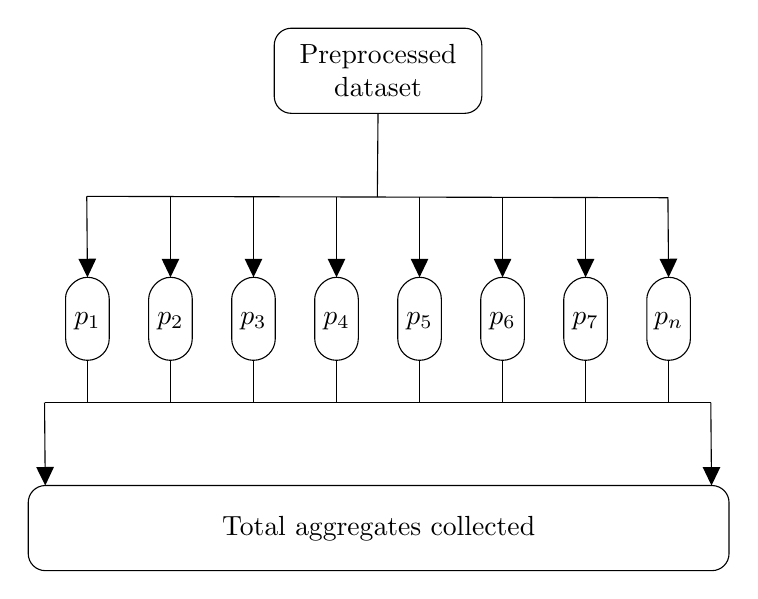
\begin{tikzpicture}[x=0.75pt,y=0.75pt,yscale=-1,xscale=1]
\draw   (290.5,47.87) .. controls (290.5,43.34) and (294.17,39.67) .. (298.7,39.67) -- (382.3,39.67) .. controls (386.83,39.67) and (390.5,43.34) .. (390.5,47.87) -- (390.5,72.47) .. controls (390.5,77) and (386.83,80.67) .. (382.3,80.67) -- (298.7,80.67) .. controls (294.17,80.67) and (290.5,77) .. (290.5,72.47) -- cycle ;
\draw    (340.5,80.67) -- (340.17,121) ;

\draw    (200.17,120.67) -- (480.17,121.33) ;
\draw    (200.17,120.67) -- (200.48,157.67) ;
\draw [shift={(200.5,159.67)}, rotate = 269.52] [fill={rgb, 255:red, 0; green, 0; blue, 0 }  ][line width=0.08]  [draw opacity=0] (8.93,-4.29) -- (0,0) -- (8.93,4.29) -- cycle    ;
\draw    (240.5,121) -- (240.5,157.67) ;
\draw [shift={(240.5,159.67)}, rotate = 270] [fill={rgb, 255:red, 0; green, 0; blue, 0 }  ][line width=0.08]  [draw opacity=0] (8.93,-4.29) -- (0,0) -- (8.93,4.29) -- cycle    ;
\draw    (280.5,121) -- (280.5,157.67) ;
\draw [shift={(280.5,159.67)}, rotate = 270] [fill={rgb, 255:red, 0; green, 0; blue, 0 }  ][line width=0.08]  [draw opacity=0] (8.93,-4.29) -- (0,0) -- (8.93,4.29) -- cycle    ;
\draw    (320.5,121) -- (320.5,156.67) ;
\draw [shift={(320.5,159.67)}, rotate = 270] [fill={rgb, 255:red, 0; green, 0; blue, 0 }  ][line width=0.08]  [draw opacity=0] (8.93,-4.29) -- (0,0) -- (8.93,4.29) -- cycle    ;
\draw    (360.5,121) -- (360.5,157.67) ;
\draw [shift={(360.5,159.67)}, rotate = 270] [fill={rgb, 255:red, 0; green, 0; blue, 0 }  ][line width=0.08]  [draw opacity=0] (8.93,-4.29) -- (0,0) -- (8.93,4.29) -- cycle    ;
\draw    (400.5,121) -- (400.5,156.67) ;
\draw [shift={(400.5,159.67)}, rotate = 270] [fill={rgb, 255:red, 0; green, 0; blue, 0 }  ][line width=0.08]  [draw opacity=0] (8.93,-4.29) -- (0,0) -- (8.93,4.29) -- cycle    ;
\draw    (440.5,121) -- (440.5,156.67) ;
\draw [shift={(440.5,159.67)}, rotate = 270] [fill={rgb, 255:red, 0; green, 0; blue, 0 }  ][line width=0.08]  [draw opacity=0] (8.93,-4.29) -- (0,0) -- (8.93,4.29) -- cycle    ;
\draw    (480.17,121) -- (480.47,156.67) ;
\draw [shift={(480.5,159.67)}, rotate = 269.5] [fill={rgb, 255:red, 0; green, 0; blue, 0 }  ][line width=0.08]  [draw opacity=0] (8.93,-4.29) -- (0,0) -- (8.93,4.29) -- cycle    ;

%1
\draw   (190,169.17) .. controls (190,165.37) and (194.7,159.67) .. (200.5,159.67) -- (200.5,159.67) .. controls (206.3,159.67) and (211,164.37) .. (211,170.17) -- (211,189.17) .. controls (211,194.97) and (206.3,199.67) .. (200.5,199.67) -- (200.5,199.67) .. controls (194.7,199.67) and (190,194.97) .. (190,189.17) -- cycle ;
%2
\draw   (230,170.17) .. controls (230,165.37) and (234.7,159.67) .. (240.5,159.67) -- (240.5,159.67) .. controls (246.3,159.67) and (251,164.37) .. (251,170.17) -- (251,189.17) .. controls (251,194.97) and (246.3,199.67) .. (240.5,199.67) -- (240.5,199.67) .. controls (234.7,199.67) and (230,194.97) .. (230,189.17) -- cycle ;
%3
\draw   (270,170.17) .. controls (270,165.37) and (274.7,159.67) .. (280.5,159.67) -- (280.5,159.67) .. controls (286.3,159.67) and (291,164.37) .. (291,170.17) -- (291,189.17) .. controls (291,194.97) and (286.3,199.67) .. (280.5,199.67) -- (280.5,199.67) .. controls (274.7,199.67) and (270,194.97) .. (270,189.17) -- cycle ;
%4
\draw   (310,170.17) .. controls (310,165.37) and (314.7,159.67) .. (320.5,159.67) -- (320.5,159.67) .. controls (326.3,159.67) and (331,164.37) .. (331,170.17) -- (331,189.17) .. controls (331,194.97) and (326.3,199.67) .. (320.5,199.67) -- (320.5,199.67) .. controls (314.7,199.67) and (310,194.97) .. (310,189.17) -- cycle ;
%5%
\draw   (350,170.17) .. controls (350,165.37) and (354.7,159.67) .. (360.5,159.67) -- (360.5,159.67) .. controls (366.3,159.67) and (371,164.37) .. (371,170.17) -- (371,189.17) .. controls (371,194.97) and (366.3,199.67) .. (360.5,199.67) -- (360.5,199.67) .. controls (354.7,199.67) and (350,194.97) .. (350,189.17) -- cycle ;
%6
\draw   (390,170.17) .. controls (390,165.37) and (394.7,159.67) .. (400.5,159.67) -- (400.5,159.67) .. controls (406.3,159.67) and (411,164.37) .. (411,170.17) -- (411,189.17) .. controls (411,194.97) and (406.3,199.67) .. (400.5,199.67) -- (400.5,199.67) .. controls (394.7,199.67) and (390,194.97) .. (390,189.17) -- cycle ;
%7
\draw   (430,170.17) .. controls (430,165.37) and (434.7,159.67) .. (440.5,159.67) -- (440.5,159.67) .. controls (446.3,159.67) and (451,164.37) .. (451,170.17) -- (451,189.17) .. controls (451,194.97) and (446.3,199.67) .. (440.5,199.67) -- (440.5,199.67) .. controls (434.7,199.67) and (430,194.97) .. (430,189.17) -- cycle ;
%n
\draw   (470,170.17) .. controls (470,165.37) and (474.7,159.67) .. (480.5,159.67) -- (480.5,159.67) .. controls (486.3,159.67) and (491,164.37) .. (491,170.17) -- (491,189.17) .. controls (491,194.97) and (486.3,199.67) .. (480.5,199.67) -- (480.5,199.67) .. controls (474.7,199.67) and (470,194.97) .. (470,189.17) -- cycle ;

\draw    (200.5,220) -- (200.5,200) ;
\draw    (240.5,220) -- (240.5,200) ;
\draw    (280.5,220) -- (280.5,200) ;
\draw    (320.5,220) -- (320.5,200) ;
\draw    (360.5,220) -- (360.5,200) ;
\draw    (400.5,220) -- (400.5,200) ;
\draw    (440.5,220) -- (440.5,200) ;
\draw    (480.5,220) -- (480.5,200) ;
\draw    (179.83,220) -- (500.83,220) ;
\draw    (179.83,220) -- (180.14,257) ;
\draw [shift={(180.17,260)}, rotate = 269.52] [fill={rgb, 255:red, 0; green, 0; blue, 0 }  ][line width=0.08]  [draw opacity=0] (8.93,-4.29) -- (0,0) -- (8.93,4.29) -- cycle    ;
\draw    (500.83,220) -- (501.14,257) ;
\draw [shift={(501.17,260)}, rotate = 270] [fill={rgb, 255:red, 0; green, 0; blue, 0 }  ][line width=0.08]  [draw opacity=0] (8.93,-4.29) -- (0,0) -- (8.93,4.29) -- cycle    ;
\draw   (171.97,268.2) .. controls (171.97,263.67) and (175.64,260) .. (180.17,260) -- (501.41,260) .. controls (505.94,260) and (509.61,263.67) .. (509.61,268.2) -- (509.61,292.8) .. controls (509.61,297.33) and (505.94,301) .. (501.41,301) -- (180.17,301) .. controls (175.64,301) and (171.97,297.33) .. (171.97,292.8) -- cycle ;
\draw (200.5,180.67) node   {$p_{1}$};
\draw (240.5,180.67) node   {$p_{2}$};
\draw (280.5,180.67) node   {$p_{3}$};
\draw (320.5,180.67) node   {$p_{4}$};
\draw (360.5,180.67) node   {$p_{5}$};
\draw (400.5,180.67) node   {$p_{6}$};
\draw (440.5,180.67) node   {$p_{7}$};
\draw (480.5,180.67) node   {$p_{n}$};
\draw (340.5,60.17) node  [align=center] {Preprocessed\\dataset};
\draw (340.79,280.5) node  [align=center] {Total aggregates collected};
\end{tikzpicture}
\caption{Performing Aggregations on Spark}
\label{partitioning}
\end{figure}

\begin{table}[htp]
\begin{adjustbox}{width=\textwidth, center}
\begin{tabular}{|c|c|c|c|c|c|c|c|c|c|c|c|}
\hline
Edu & Edu\_Gen & Edu\_Child\_Gen & Edu\_Any & Edu\_Any\_Y & Edu\_Any\_N & Edu\_WPS & Edu\_PS & Edu\_WPS\_Y & Edu\_WPS\_N & Edu\_PS\_Y & Edu\_PS\_N\\
\hline
9th & Any & WPS & 3 & 0 & 3 & 3 & 0 & 0 & 3 & 0 & 0\\
10th & Any & WPS & 4 & 0 & 4 & 4 & 0 & 0 & 4 & 0 & 0\\
11th & Any & WPS & 5 & 2 & 3 & 5 & 0 & 2 & 3 & 0 & 0\\
12th & Any & WPS & 4 & 3 & 1 & 4 & 0 & 3 & 1 & 0 & 0\\
Bachelors & Any & PS & 6 & 4 & 2 & 0 & 6 & 0 & 0 & 4 & 2\\
Bachelors & Any & PS & 4 & 4 & 0 & 0 & 4 & 0 & 0 & 4 & 0\\
Masters & Any & PS & 4 & 4 & 0 & 0 & 4 & 0 & 0 & 4 & 0\\
Masters & Any & PS & 3 & 3 & 0 & 0 & 3 & 0 & 0 & 3 & 0\\
Doctorate & Any & PS & 1 & 1 & 0 & 0 & 1 & 0 & 0 & 1 & 0\\
\hline
\end{tabular}
\end{adjustbox}
\caption{Education Transformation}
\label{table3}
\end{table}

Once we have all the transformations, we can then perform the aggregations that will provide us with the total numbers to be used in the score calculation equations. The aggregation dataset is just one row with all the aggregates as shown in Table~\ref{table4}. The values for the aggregates correspond to the same values in the example provided in Section~\ref{tdsIntro}. Spark performs these aggregations in parallel for every partition. The aggregation is followed by a $collect$ call which triggers Spark to collect all the aggregates from the worker nodes into the master node which then gets stored in a local variable representing Table~\ref{table4}. The scores are then calculated using the local variable. The highest scoring $AC$ (Anonymization Cut) tree is selected, its root is removed from the $AC$ set, and its children's subtrees are added. The dataset is then generalized to the root of all respective $AC$ trees, $k$ is calculated, and the iteration continues until $k$ is violated. The main algorithm can be summarized in Algorithm~\ref{tdsImplemented} above.

\begin{table}[htp]
\begin{adjustbox}{width=\textwidth, center}
\begin{tabular}{|c|c|c|c|c|c|c|c|c|}
\hline
Edu\_Any & Edu\_Any\_Y & Edu\_Any\_N & Edu\_WPS & Edu\_PS & Edu\_WPS\_Y & Edu\_WPS\_N & Edu\_PS\_Y & Edu\_PS\_N\\
\hline
34 & 21 & 13 & 16 & 18 & 5 & 11 & 16 & 2\\
\hline
\end{tabular}
\end{adjustbox}
\caption{Education Aggregation}
\label{table4}
\end{table}

The path map that gets returned from Algorithm~\ref{tdsImplemented} Line~\ref{originalPathMap} or \ref{newMap} once it is done can be as follows:

\begin{verbatim}
education:
    Map(
        7th-8th: Queue(Elementary, 7th-8th),
        Bachelors: Queue(University, Bachelors),
        ...
    ),
native-country:
    Map(
        Vietnam: Queue(Asia, Southeastern-Asia, Vietnam),
        ...
    ),
...
\end{verbatim}

This anonymization map can then be passed to a Spark User Defined Function (UDF) that gets executed on every cell. For education column it will generalize \emph{7th-8th} values to \emph{Elementary} and \emph{Bachelors} to \emph{University}. For native country column, \emph{Vietnam} values will be generalized to \emph{Asia}

\subsection{Performance enhancements}

Multiple considerations have been taken into account in order to improve performance. The first was generating path maps from taxonomy trees in the preprocessing step in order to speed up tree lookups performed during generalization. I also had to perform multiple experiments with a variety of different partition numbers in order to achieve the best performance. The best performance was achieved when number of partitions was set to total number of cores in the cluster. This finding corroborates findings of \cite{Sopaoglu:2017}. Tail recursion was also preferred over looping as a performance enhancement technique. Dataset was also partitioned over an arbitrary unique $rowId$ assigned to every row in the preprocessing stage. When partitioning is left completely up to Spark by only providing the number of partitions, it was found that this does not guarantee an equally distributed number of partitions across all worker nodes. An even distribution was achieved by partitioning over a unique ID column as well as providing the number of partitions.

Lastly, the biggest improvement enhancement was achieved by performing the aggregations of all taxonomy trees at once, in parallel, and then collecting the total aggregates to a local variable. The brute-force attempt of the implementation was only performing the aggregations of individual $QID$s in parallel and then collecting aggregates for each $QID$ separately. By doing all aggregations of all taxonomy trees in parallel, which essentially reduced aggregations and collect calls to only one per iteration, runtime was reduced from 4 hours to 15 minutes on a 5-million row dataset in an 8-node cluster. In Section~\ref{evaluation} I review those performance results in detail.

% usage: \includeFig{label}{file}{caption}

% ############################################################################
\section{Experimental Evaluation} \label{evaluation}
% ############################################################################

Experiments were performed on an OpenStack cluster with 1, 2, 4, 8 and 16 worker nodes. Each node had 4 vCPUs, 8 GB RAM and 32 GB disk size. All nodes were running Spark version 2.4.2, Scala 12.10 and Java 8. The dataset used is the same \emph{Adult} dataset referenced in \cite{Sopaoglu:2017} however it was enlarged to 4 different datasets of 250,000, 5 million, 10 million and 20 million-row datasets. The enlargement process involved writing a program to inject rows using a random value from the list of distinct values in the original dataset for every column.

A total of 8 $QID$ values were specified. All were categorical attributes: $education$, $marital\_status$, $occupation$, $native\_country$, $workclass$, $relationship$, $race$, $sex$. The $k$ value was set to 100.

The first experiment was determining the number of partitions. Using a 5 million dataset and running on an 8-node cluster, the following variations were tested for number of partitions: 16, 32 (total number of vCPUs in the cluster), 50, 100, 200 (Spark's default number of partitions), 300, 400 and 528. As shown in Figure~\ref{bestPartition}, the best performance was when number of partitions set to the number of total vCPUs in the cluster which performed 1.5 times faster than the Spark default. The dashed vertical line represents the best performing and the dotted represents Spark's default. The most likely explanation is that when partitions are fewer than number of CPUs, not all cores are utilized. While when the number of partitions is much higher than number of cores, the partitioned dataset becomes too small to the point that the overhead of partitioning exceeds the time it takes to execute the task itself.

\begin{figure}[htp]
\centering
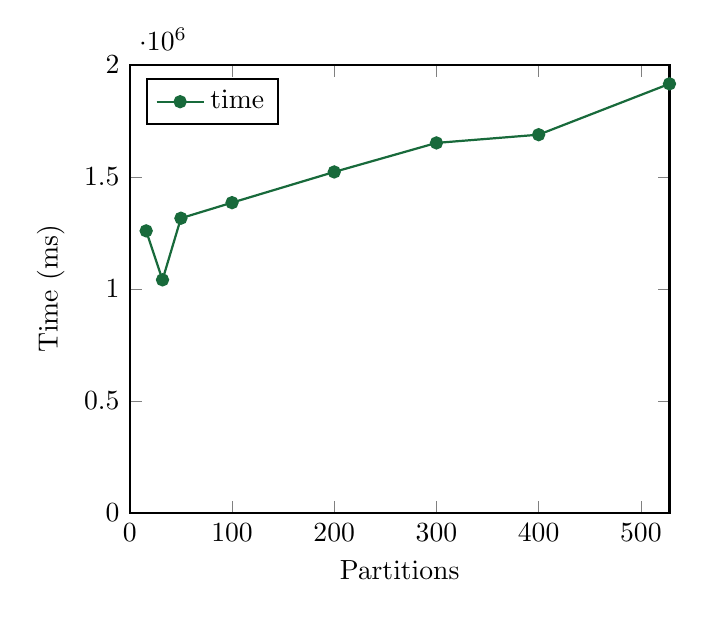
\begin{tikzpicture}
\begin{axis}[
    xlabel={Partitions},
    ylabel={Time (ms)},
    xmin=0, xmax=528,
    ymin=0, ymax=2000000,
    legend pos=north west,
    grid style=dashed,
    style=thick
]

\addplot[color=darkGreen,mark=*]
coordinates {(16,1258976)(32,1040411)(50,1315358)(100,1384842)(200,1521808)(300,1651312)(400,1688017)(528,1914883)};

\draw [dashed] (32,0) -- (32,165);
\draw [dotted] (200,0) -- (200,165);

\legend{time}
\end{axis}
\end{tikzpicture}
\caption{Determining Best Number of Partitions}
\label{bestPartition}
\end{figure}

The following experiment evaluated the scale-up of Top-Down Specialization on Spark shown in Figure~\ref{scaleUp}. Running 4 different datasets on a 16-node cluster and 64 partitions, we can see that when the dataset size increases by 100\% from 5 to 10 to 20 million, the runtime only increases by 55-65\%

\begin{figure}[h]
\centering
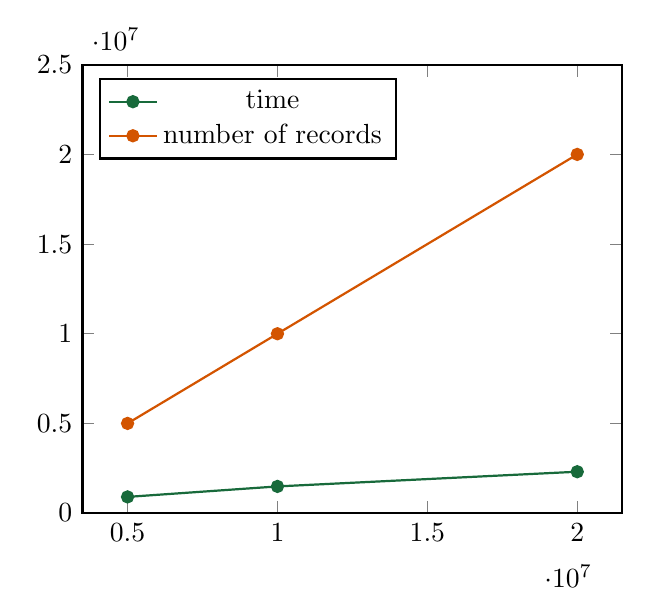
\begin{tikzpicture}
\begin{axis}[
    ymin=0, ymax=25000000,
    legend pos=north west,
    grid style=dashed,
    style=thick
]

\addplot[color=darkGreen,mark=*]
coordinates {(5000000,901938)(10000000,1486063)(20000000,2305491)};

\addplot[color=orange,mark=*]
coordinates {(5000000,5000000)(10000000,10000000)(20000000,20000000)};

\legend{time, number of records}
\end{axis}
\end{tikzpicture}
\caption{Scale-up of TDS on Spark}
\label{scaleUp}
\end{figure}

We then assess the speed-up of the algorithm. Speed up experiments were conducted for datasets of 250,000 rows as well as 5, 10 and 20-million rows. As shown, the speedup significantly improved as the size of the dataset became larger. This is most likely also attributable to the partitioning overhead cost exceeding the task computation cost for smaller datasets. 


\begin{center}
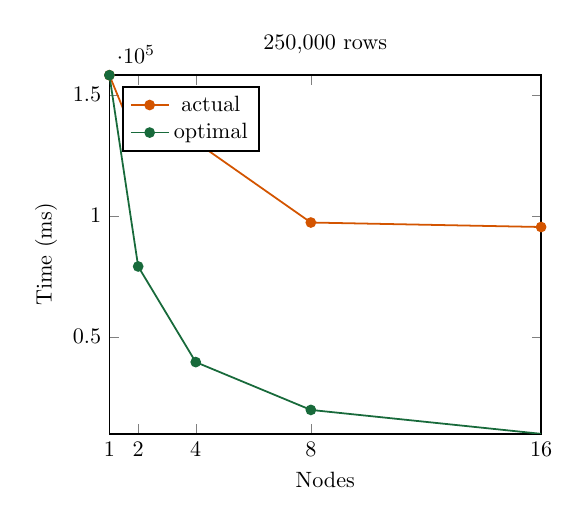
\begin{tikzpicture}[scale=0.8]
\begin{axis}[
    title={250,000 rows},
    xtick = {1,2,4,8,16},
    xlabel={Nodes},
    ylabel={Time (ms)},
    xmin=1, xmax=16,
    ymin=9881.125, ymax=158098,
    legend pos=north west,
    grid style=dashed,
    style=thick
]

\addplot[color=orange,mark=*]
coordinates {(1,158098)(2,129070)(4,130564)(8,97207)(16,95352)};

\addplot[color=darkGreen,mark=*]
coordinates {(1,158098)(2,79049)(4,39525)(8,19762)(16,9881)};

\legend{actual, optimal}
\end{axis}
\end{tikzpicture}
\hspace{1cm}
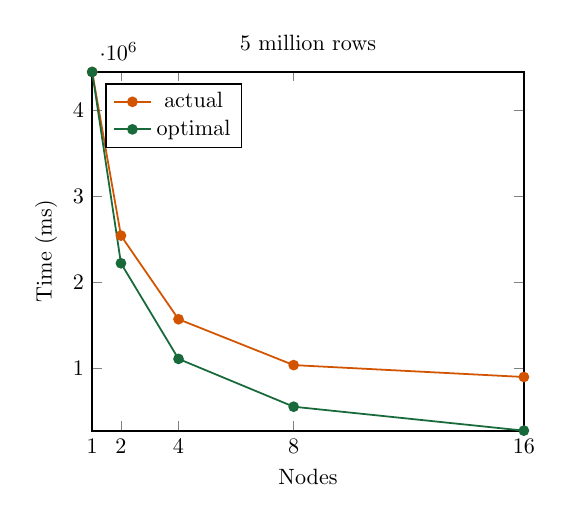
\begin{tikzpicture}[scale=0.8]
\begin{axis}[
    title={5 million rows},
    xtick = {1,2,4,8,16},
    xlabel={Nodes},
    ylabel={Time (ms)},
    xmin=1, xmax=16,
    ymin=278111, ymax=4449781,
    legend pos=north west,
    grid style=dashed,
    style=thick
]

\addplot[color=orange,mark=*]
coordinates {(1,4449781)(2,2546598)(4,1573823)(8,1040411)(16,901938)};

\addplot[color=darkGreen,mark=*]
coordinates {(1,4449781)(2,2224891)(4,1112445)(8,556223)(16,278111)};

\legend{actual, optimal}
\end{axis}
\end{tikzpicture}
\end{center}


\begin{center}
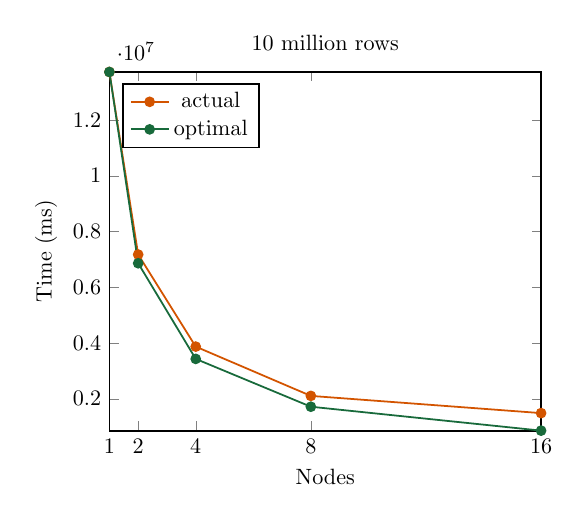
\begin{tikzpicture}[scale=0.8]
\begin{axis}[
    title={10 million rows},
    xtick = {1,2,4,8,16},
    xlabel={Nodes},
    ylabel={Time (ms)},
    xmin=1, xmax=16,
    ymin=857689, ymax=13723016,
    legend pos=north west,
    grid style=dashed,
    style=thick
]

\addplot[color=orange,mark=*]
coordinates {(1,13723016)(2,7174442)(4,3871286)(8,2103755)(16,1486063)};

\addplot[color=darkGreen,mark=*]
coordinates {(1,13723016)(2,6861508)(4,3430754)(8,1715377)(16,857689)};

\legend{actual, optimal}
\end{axis}
\end{tikzpicture}
\hspace{1cm}
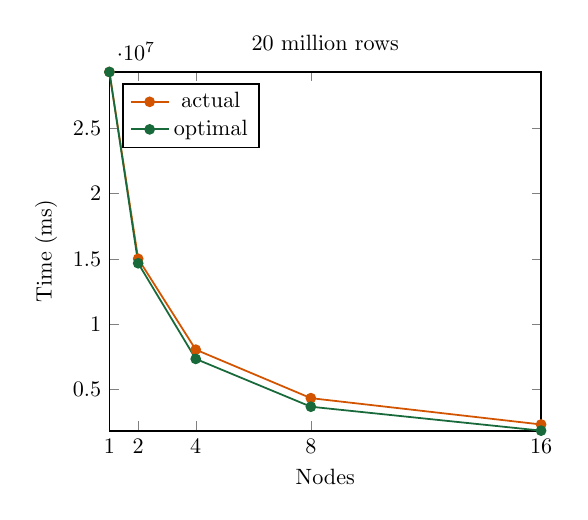
\begin{tikzpicture}[scale=0.8]
\begin{axis}[
    title={20 million rows},
    xtick = {1,2,4,8,16},
    xlabel={Nodes},
    ylabel={Time (ms)},
    xmin=1, xmax=16,
    ymin=1833101, ymax=29329618,
    legend pos=north west,
    grid style=dashed,
    style=thick
]

\addplot[color=orange,mark=*]
coordinates {(1,29329618)(2,15007906)(4,8041695)(8,4323788)(16,2305491)};

\addplot[color=darkGreen,mark=*]
coordinates {(1,29329618)(2,14664809)(4,7332405)(8,3666202)(16,1833101)};

\legend{actual, optimal}
\end{axis}
\end{tikzpicture}
\end{center}

In comparison with the original paper \cite{Sopaoglu:2017}, we can see that their speedup was slightly better for 5-million row dataset. Please note that \cite{Sopaoglu:2017} used size on disk for measurement which was equivalent to this paper's 5-million row dataset. Please also note that the test environment used in the original paper was slightly different as the authors installed Spark on Docker contains on the same 32-core machine. It is presumed that the communication between Docker images on the same machine will not have the communication overhead between workers in a cluster where this paper's implementation was tested.

\begin{center}
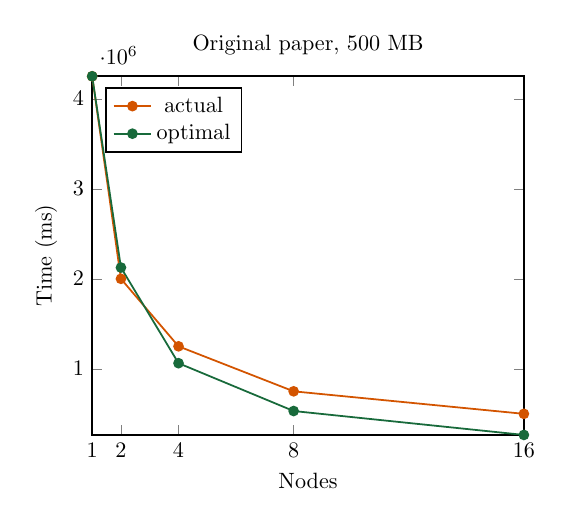
\begin{tikzpicture}[scale=0.8]
\begin{axis}[
    title={Original paper, 500 MB},
    xtick = {1,2,4,8,16},
    xlabel={Nodes},
    ylabel={Time (ms)},
    xmin=1, xmax=16,
    ymin=265625, ymax=4250000,
    legend pos=north west,
    grid style=dashed,
    style=thick
]

\addplot[color=orange,mark=*]
coordinates {(1,4250000)(2,2000000)(4,1250000)(8,750000)(16,500000)};

\addplot[color=darkGreen,mark=*]
coordinates {(1,4250000)(2,2125000)(4,1062500)(8,531250)(16,265625)};

\legend{actual, optimal}
\end{axis}
\end{tikzpicture}
\hspace{1cm}
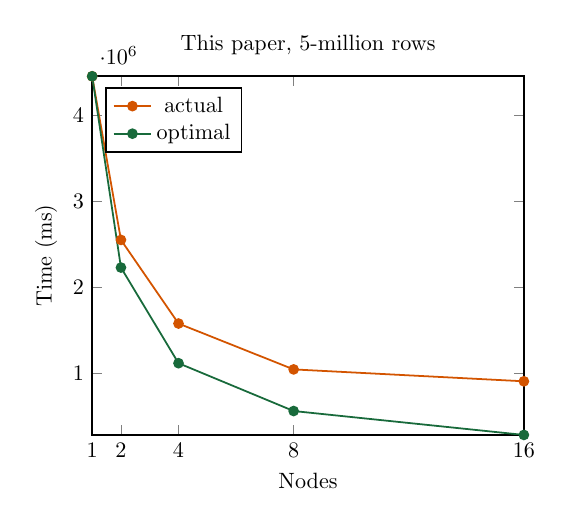
\begin{tikzpicture}[scale=0.8]
\begin{axis}[
    title={This paper, 5-million rows},
    xtick = {1,2,4,8,16},
    xlabel={Nodes},
    ylabel={Time (ms)},
    xmin=1, xmax=16,
    ymin=278111, ymax=4449781,
    legend pos=north west,
    grid style=dashed,
    style=thick
]

\addplot[color=orange,mark=*]
coordinates {(1,4449781)(2,2546598)(4,1573823)(8,1040411)(16,901938)};

\addplot[color=darkGreen,mark=*]
coordinates {(1,4449781)(2,2224891)(4,1112445)(8,556223)(16,278111)};

\legend{actual, optimal}
\end{axis}
\end{tikzpicture}
\end{center}

Finally, another test was performed on a 32-core machine and 128 GB RAM for the 10-million row dataset. As shown, the 10-million row running on a cluster had a much better speedup compared to the same dataset running in a 32-core machine. The most likely reason for this is as the dataset increases, the bus communication traffic becomes congested which serves as a bottleneck not present in a cluster environment. Spark documentation also shows that running locally on the same machine is meant for testing only and some out-of-the-box Spark performance enhancements are only available for cluster environments.

\begin{center}
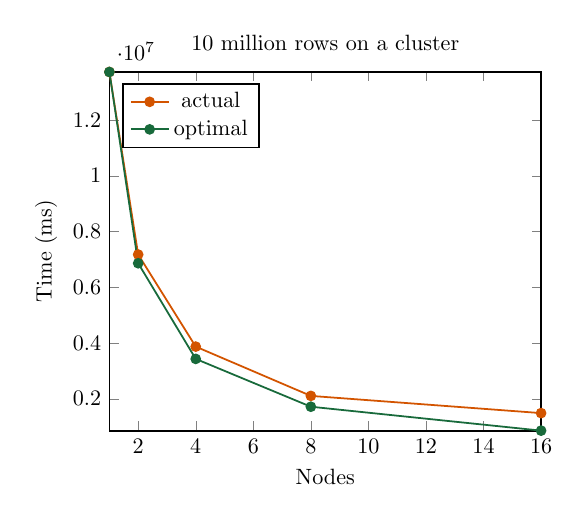
\begin{tikzpicture}[scale=0.8]
\begin{axis}[
    title={10 million rows on a cluster},
    xlabel={Nodes},
    ylabel={Time (ms)},
    xmin=1, xmax=16,
    ymin=857689, ymax=13723016,
    legend pos=north west,
    grid style=dashed,
    style=thick
]

\addplot[color=orange,mark=*]
coordinates {(1,13723016)(2,7174442)(4,3871286)(8,2103755)(16,1486063)};

\addplot[color=darkGreen,mark=*]
coordinates {(1,13723016)(2,6861508)(4,3430754)(8,1715377)(16,857689)};

\legend{actual, optimal}
\end{axis}
\end{tikzpicture}
\hspace{1cm}
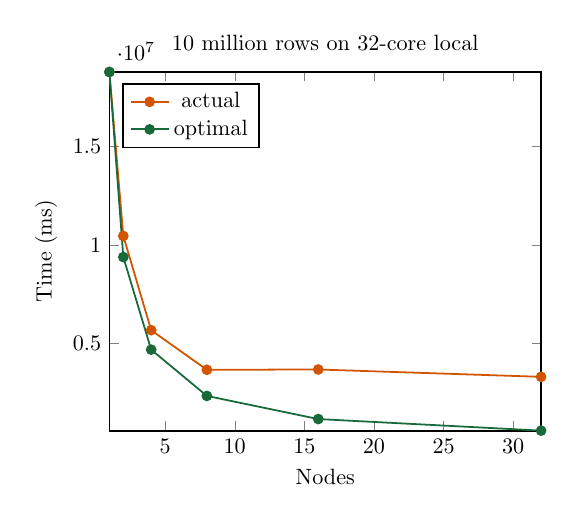
\begin{tikzpicture}[scale=0.8]
\begin{axis}[
    title={10 million rows on 32-core local},
    xlabel={Nodes},
    ylabel={Time (ms)},
    xmin=1, xmax=32,
    ymin=586845, ymax=18779043,
    legend pos=north west,
    grid style=dashed,
    style=thick
]

\addplot[color=orange,mark=*]
coordinates {(1,18779043)(2,10458207)(4,5681087)(8,3670931)(16,3688598)(32,3315245)};

\addplot[color=darkGreen,mark=*]
coordinates {(1,18779043)(2,9389522)(4,4694761)(8,2347380)(16,1173690)(32,586845)};

\legend{actual, optimal}
\end{axis}
\end{tikzpicture}
\end{center}

% ############################################################################
\section{Conclusions} \label{conclusion}
% ############################################################################

Based on experiments conducted in Section~\ref{evaluation}, I can conclude the following:

\subsection{Conclusions}

This paper's implementation had speedups close to optimal for larger datasets of 20-million rows. The scale up curve was also virtually flat; when dataset size doubled, runtime only increased by half. In order to achieve the best performance, Spark partitions need to equal total number of cores in a cluster. Top-Down Specialization on Spark also performed better in a cluster environment compared to local machines even when locally the cores were more powerful than on the cluster. For iterative algorithms, minimizing the number of aggregations and collection from worker nodes to only one yields the best performance results. Even when the aggregations are performed on wide tables of $\approx$100 columns.

\subsection{Summary of Contributions}

This paper enhanced the preprocessing stage by implementing an algorithm that built path maps from taxonomy trees. This provided the option of performing look-ups in constant time during the iterations. It also evaluated the performance of Top-Down Specialization algorithm on Spark on datasets up to 4-times larger than tested in \cite{Sopaoglu:2017}. Evaluations of the algorithm were also made in a cluster environment which is more typical for production applications.

\subsection{Future Research}

The Top-Down Specialization algorithm starts by generalizing all values to the root of taxonomy trees. This introduces redundant iterations for larger datasets as it will iterate all the way from \(k=n\) where $n$ is the number of records to a much lower number such as \(k=100\). Future research can enhance algorithms such as Hybrid Top-Down and Bottom-Up algorithm proposed in \cite{Zhang:2013} by adapting it for Spark. It is also worth researching starting the generalization at a level deeper than the root to avoid these redundant iterations. 

% ############################################################################
% Bibliography
% ############################################################################
\bibliographystyle{plain}
\bibliography{my-bibliography}     %loads my-bibliography.bib

% ============================================================================
\end{document}
% ============================================================================
